%!TEX root = ../main.tex
\section{An Overview of DeepEye}
\label{sec:system}

\subsection{System Architecture}

%\add{Rename the layers to be consistent with Introduction.}
We present \sys, an end-to-end framework to prepare data, select visualizations and allow easy-to-use interactions. An overview of \sys is given in Figure~\ref{fig:framwork}, which consists of three layers: {\em (task-driven) data preparation layer}, {\em (smart) data analytics layer}, and {\em user interaction layer}.
%
%\add{!!!!}
%
Data preparation is responsible for crawling daily updated data from different sources, and cleaning them when needed (Section~\ref{subsec:dp}).
%
Data analytics describes the process of both which charts will always be shown (\eg a heat map on a world map showing new cases of every country), and how to automatically recommend visualizations that are ``interesting'' \wrt new incoming data, for visual analytics (Section~\ref{subsec:vs}).
%
Interaction allows a user to explore various and (maybe) new COVID-19 stories in an interactive fashion (Section~\ref{subsec:ie}).


\subsection{Task-driven Data Preparation Layer}
\label{subsec:dp}

%%%%%%%%%%%%%%%%%%%%%%%%%%%%%%%%%%%%
\begin{figure}[t!]
	\centering
	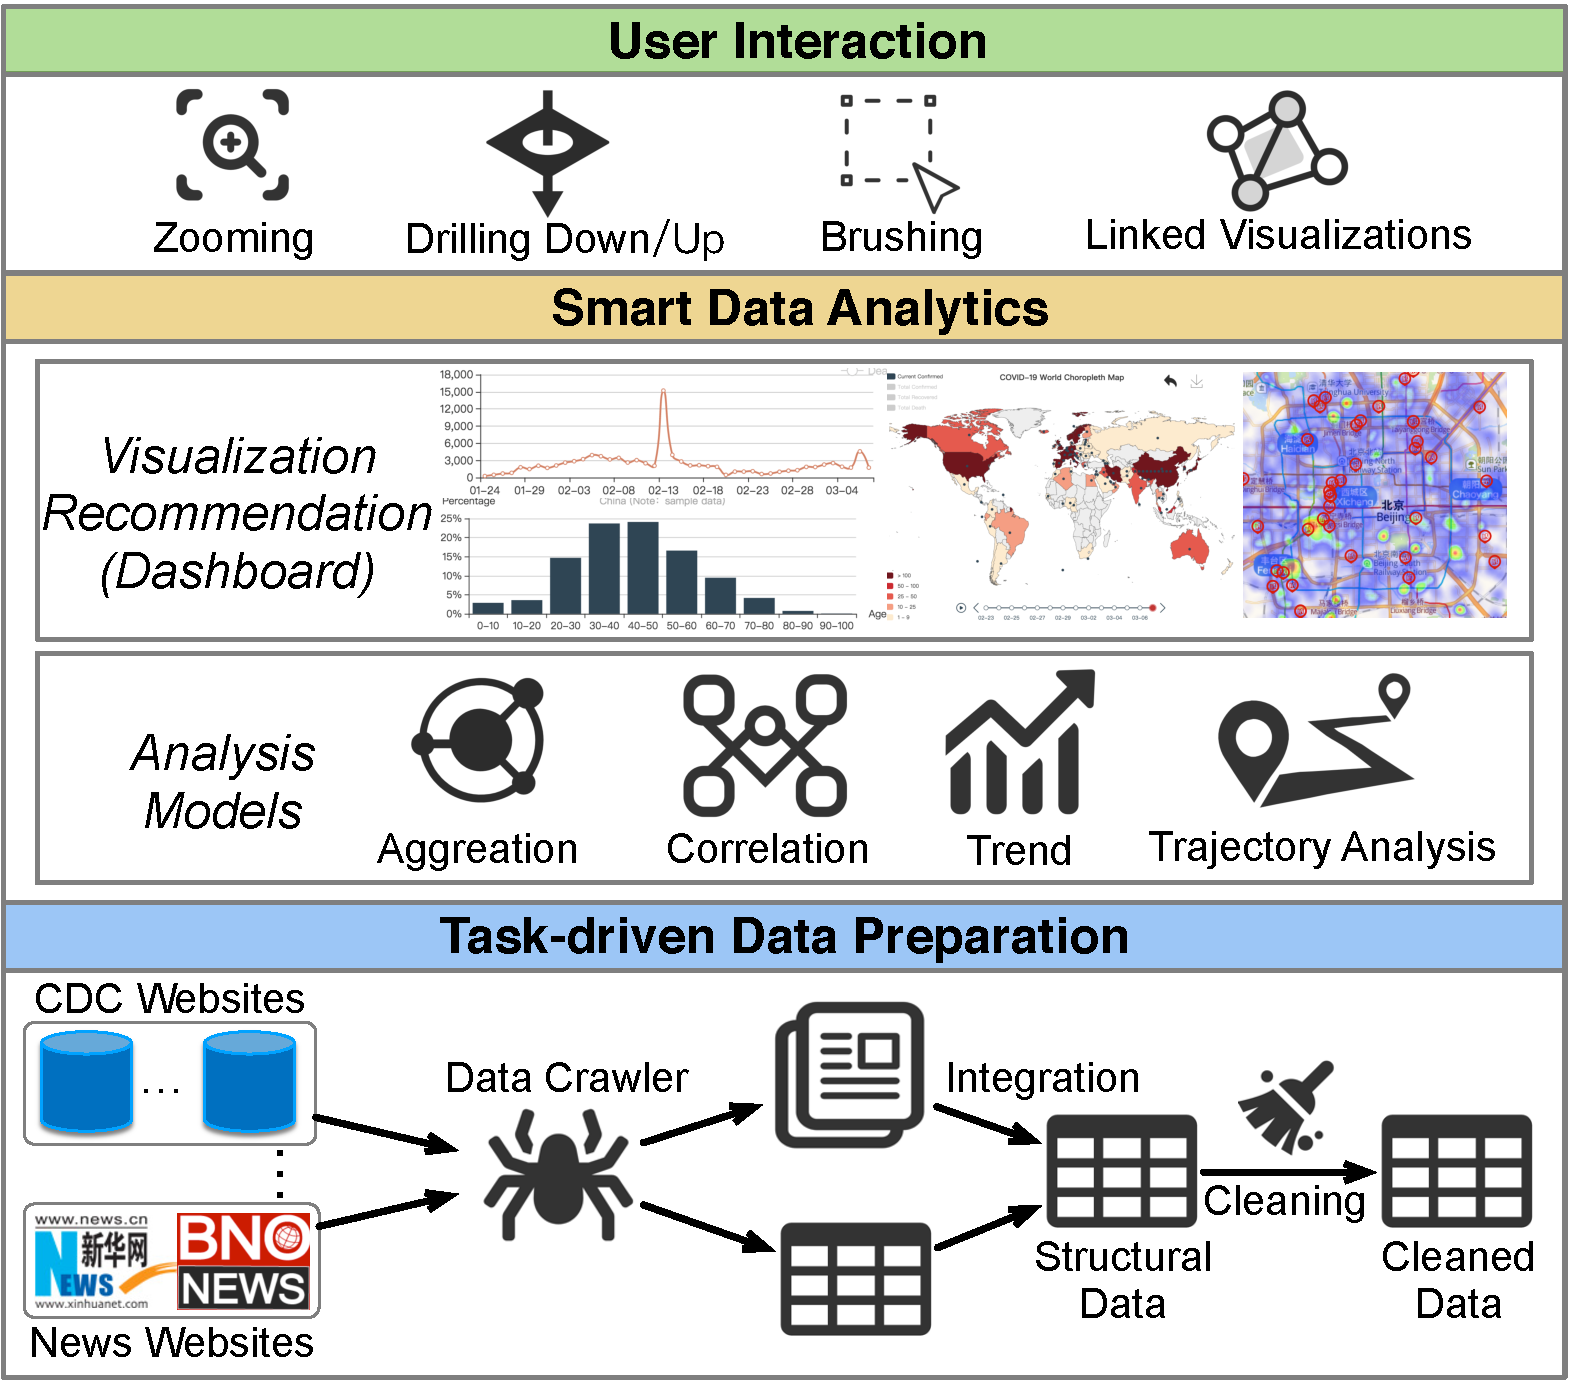
\includegraphics[width=.6\columnwidth]{figs/framework.pdf}
	\caption{System Overview}
	\label{fig:framwork}
\end{figure}
%%%%%%%%%%%%%%%%%%%%%%%%%%%%%%%%%%%%


This layer has a predefined pipeline to prepare data, which will run periodically, with the following three steps.

\stitle{Data Collection.}
We collect data from the following data sources.
(1) We download hourly the official data from the Chinese Center for Disease Control and Prevention (CDC) and other countries' CDCs.
(2) We crawl infected cases' age and gender from authoritative news websites.
(3) We also connect to other data sources like population statistics, temperature data, and so on. 
(4) We are also provided with trajectory data of (potentially) infected persons from China Mobile Limited\footnote{We are collaborating with the company and got mobile phone location data under privacy protection.}. 
%The schema is {\sf S1:}({\sf PhoneID}, {\sf Tag}, {\sf Province}, {\sf City}, {\sf District}, {\sf Address}, { \sf Longitude}, {\sf Latitude}, {\sf Time}).

\stitle{Data Integration.} Next, we need to integrate different types of data into predefined relational tables (\ie global views).
For example, we need to extract report date, location, patients' type, \#-cases from each country's CDC's reports, and  perform schema alignment into  $S1$: ({\em Date, Country, State/Province, City, Total Confirmed, Active Confirmed, Total Deaths, Total Recovered, Death Rate, Recovered Rate, Gender)}, a typical ETL-based data integration process. 


\stitle{Data Cleaning.} After integrating data from multiple sources, there have typical data errors such as duplicates, missing values, synonyms, and so on. 
%\add{Add a sentence to say that we will discuss task-driven data cleaning in Section 3.}
Because data cleaning is known to be tedious and error-prone, we employ our recently proposed technique {\sc VisClean}~\cite{visclean-icde} for visualization-aware data cleaning, which is way cheaper than cleaning the entire dataset. This is doable only after the charts to display have been selected, as discussed below. 
We will depict more details about visualization-aware data cleaning in Section~\ref{sec:dataprep}.

\subsection{Smart Data Analytics Layer}
\label{subsec:vs}
Based on the availability and reliability of data and meta-data, we have successfully conducted the following types of data analytics.

\stitle{Descriptive analytics.} 
We use linked data visualization and visualization recommendation algorithms to effectively show what happened in the past.


\stitle{Diagnostic analytics.} 
We use maps with different layers to test the spatio-temporal properties of COVID-19 data, especially to show the effect of urban (population) density and temperature to the outbreak of COVID-19.


\stitle{Prescriptive analytics.}
Based on the collaboration with companies to get private data, we were able to do some meaningful prescriptive analytics that can recommend actions to decision makers.

%%%%%%%%%%%%%%%%%%%%%%%%%%%%%%%%%%%%
%\begin{figure}[t!]
%	\centering
%	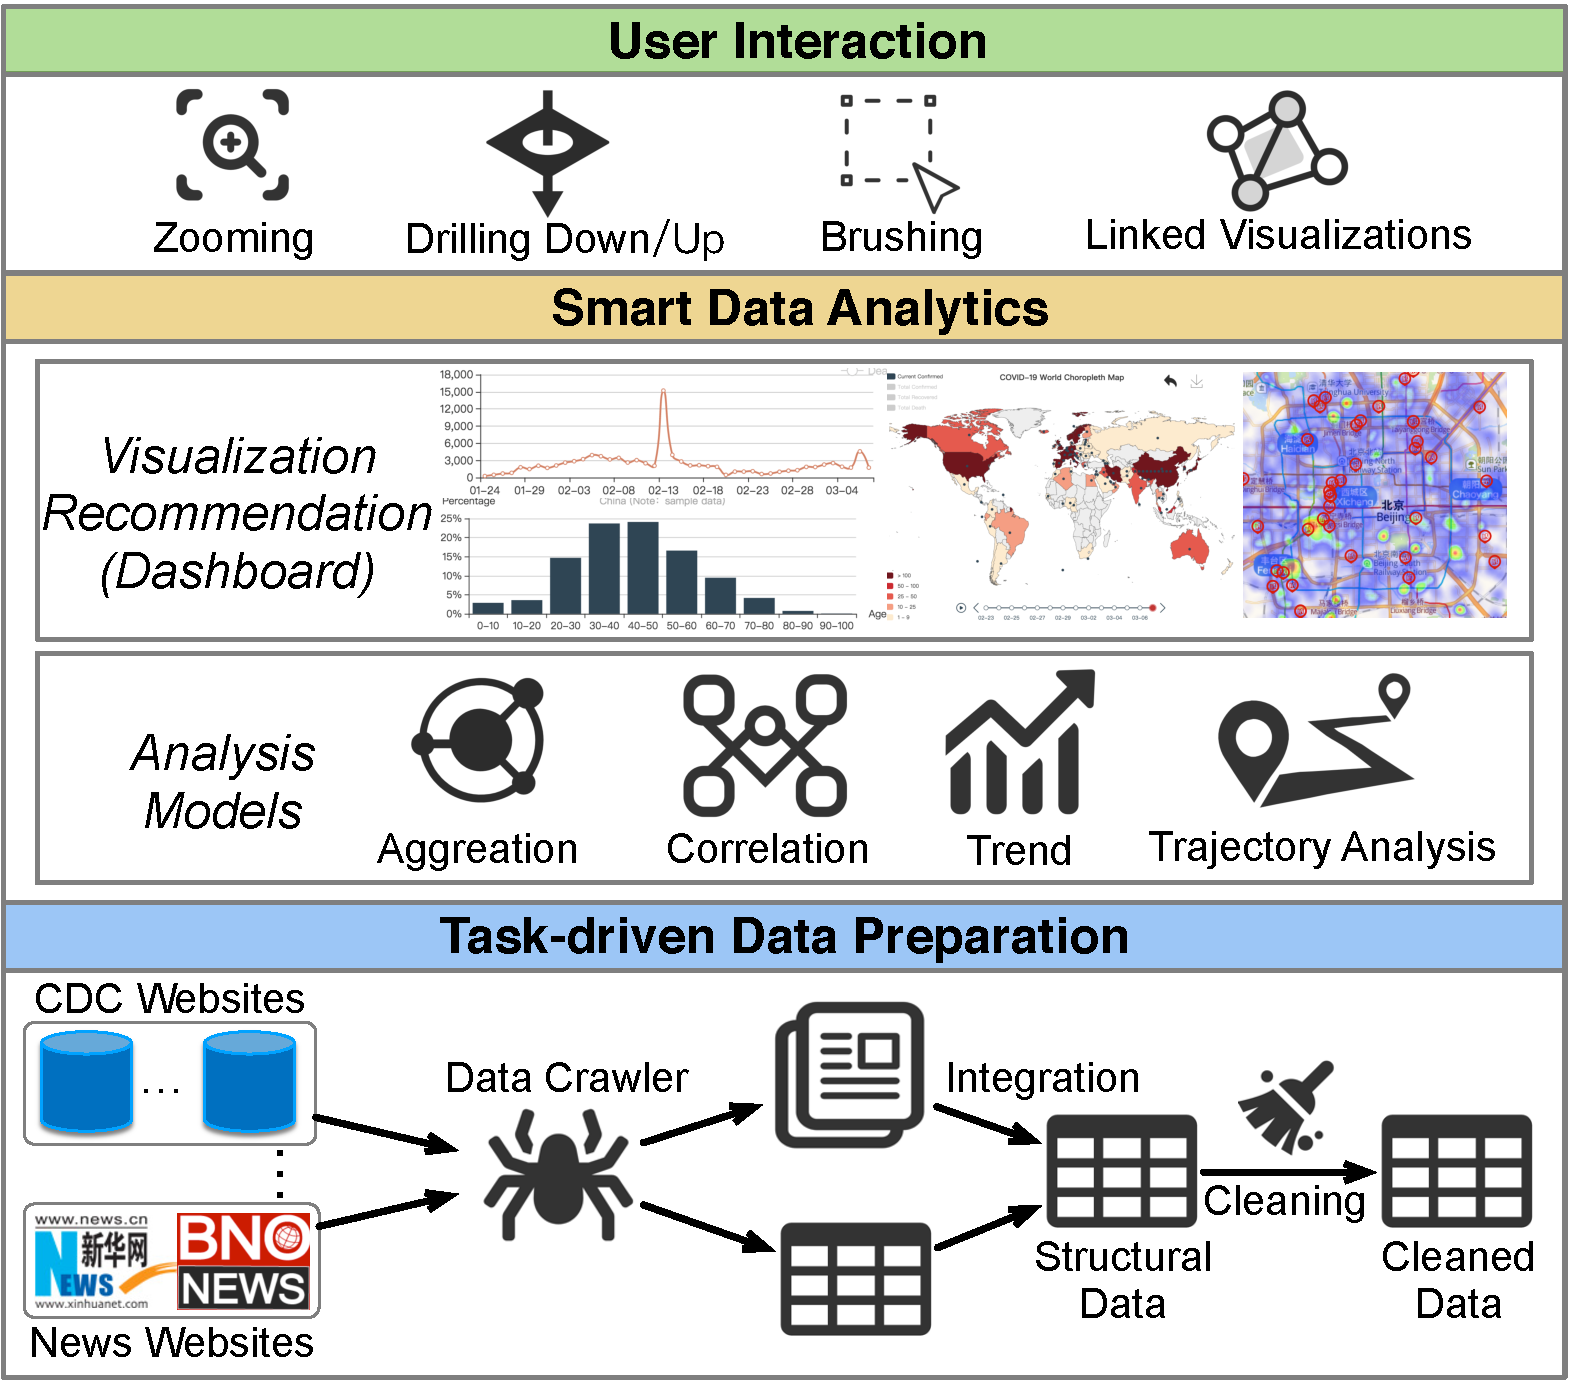
\includegraphics[width=.6\columnwidth]{figs/framework.pdf}
%	%	\vspace{-1.5em}
%	\caption{System Overview}
%	\label{fig:framwork}
%	%	\vspace{-2.5em}
%\end{figure}
%%%%%%%%%%%%%%%%%%%%%%%%%%%%%%%%%%%%





%%%%%%%%%%%%%%%%%%%%%%%%%%%%%%%%%%%%
%\begin{figure*}[t!]
%	\vspace{-1.5em}
%	\centering
%	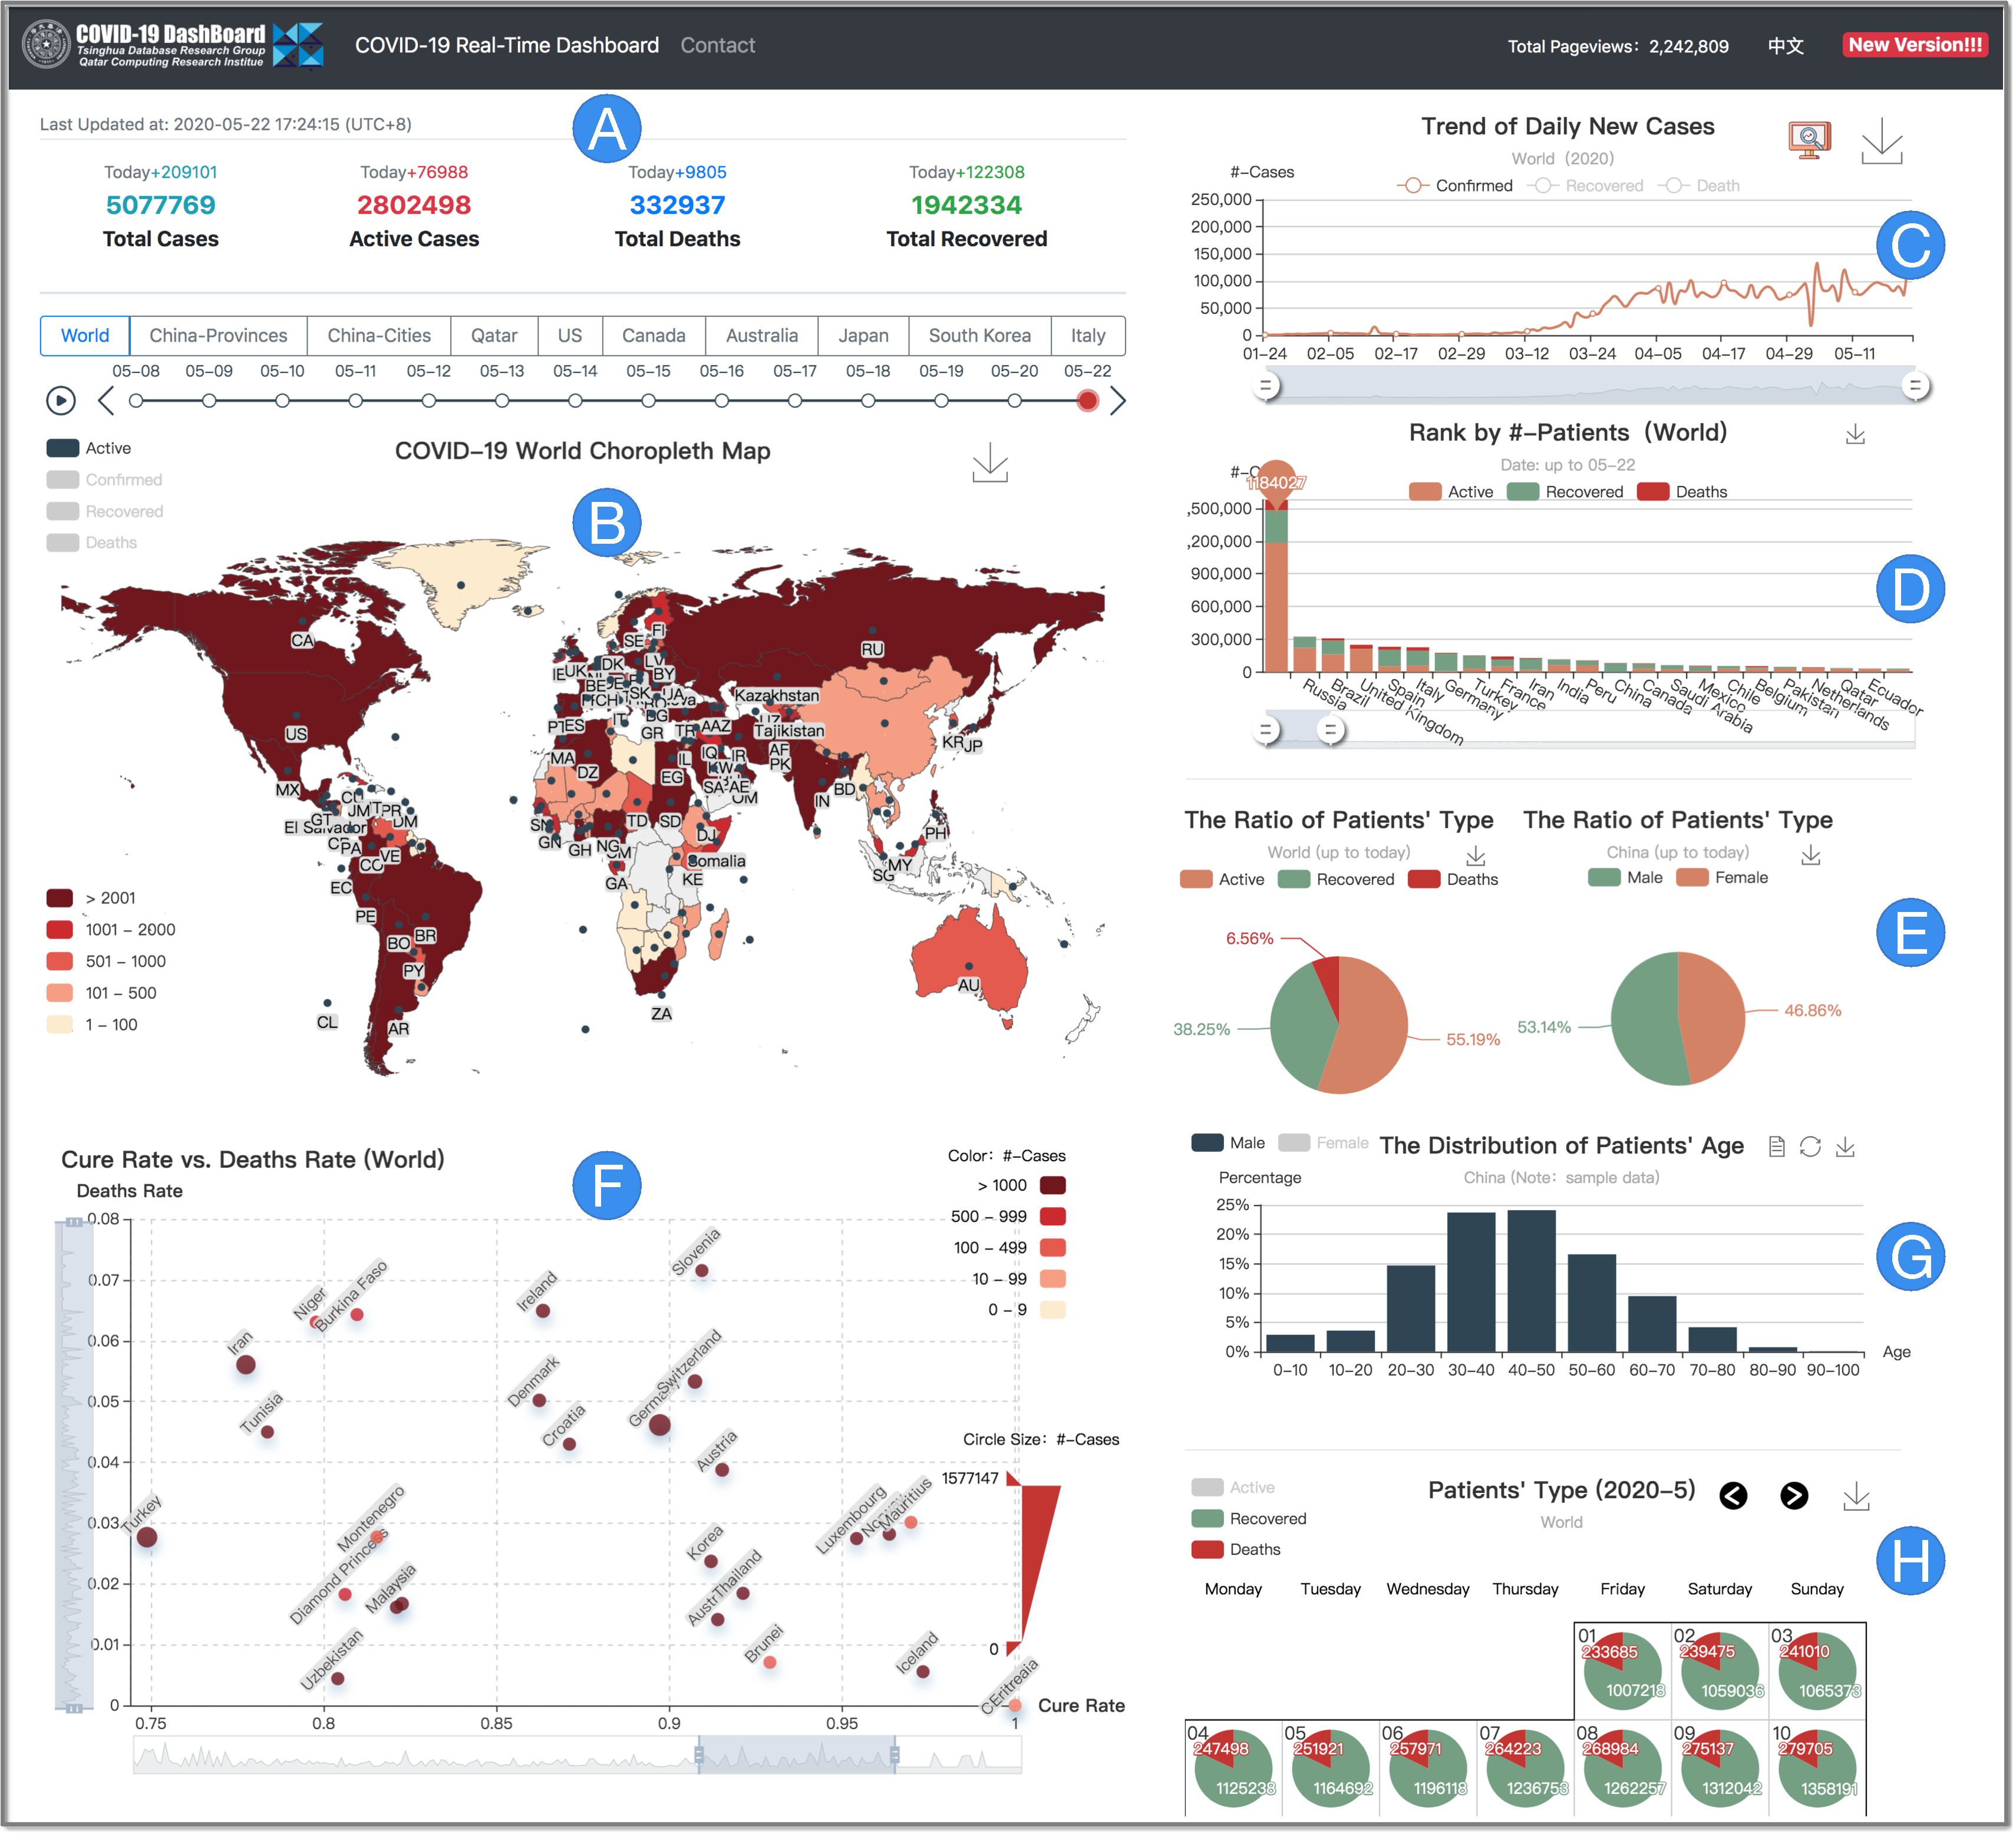
\includegraphics[width=0.9\textwidth]{figs/frontend.pdf}
%	%	\vspace{-1.5em}
%	\caption{Demonstration of \sys-COVID-19 (https://ncov.deepeye.tech/en)}
%	\label{fig:frontend}
%	%	\vspace{-1.5em}
%\end{figure*}
%%%%%%%%%%%%%%%%%%%%%%%%%%%%%%%%%%%%


% \stitle{\sys-COVID-19:}
% We have implemented a \sys instance for COVID-19, which has attracted a broad range of interest from general users, public health authorities, and researchers who want to explore the COVID-19 data and track the outbreak. 
% %


% The base view of \sys-COVID-19 is shown in Figure~\ref{fig:frontend}, which consists of a choropleth map for the total confirmed/recovered/died cases for all countries, line charts for the trend of daily increased cases, calendar charts for visualizing the types of patients, bar charts for distributions of patients' ages, bubble charts for cure rate - death rate, and so on. 
% %
% Besides the basic view page, it also has ad-hoc features, such as tracking infection path and high-risk areas discovery using the trajectory data of infected persons, which will be discussed in Section~\ref{sec:demo}.


% \sys has three layers (see Figure~\ref{fig:framwork}): (1) data preparation, (2) visualization selection, and (3) interaction.
% Next, we will explain each step using the COVID-19 case.


% %%%%%%%%%%%%%%%%%%%%%%%%%%%%%%%%%%%%
% \begin{figure*}[t!]
% 	\centering
% 	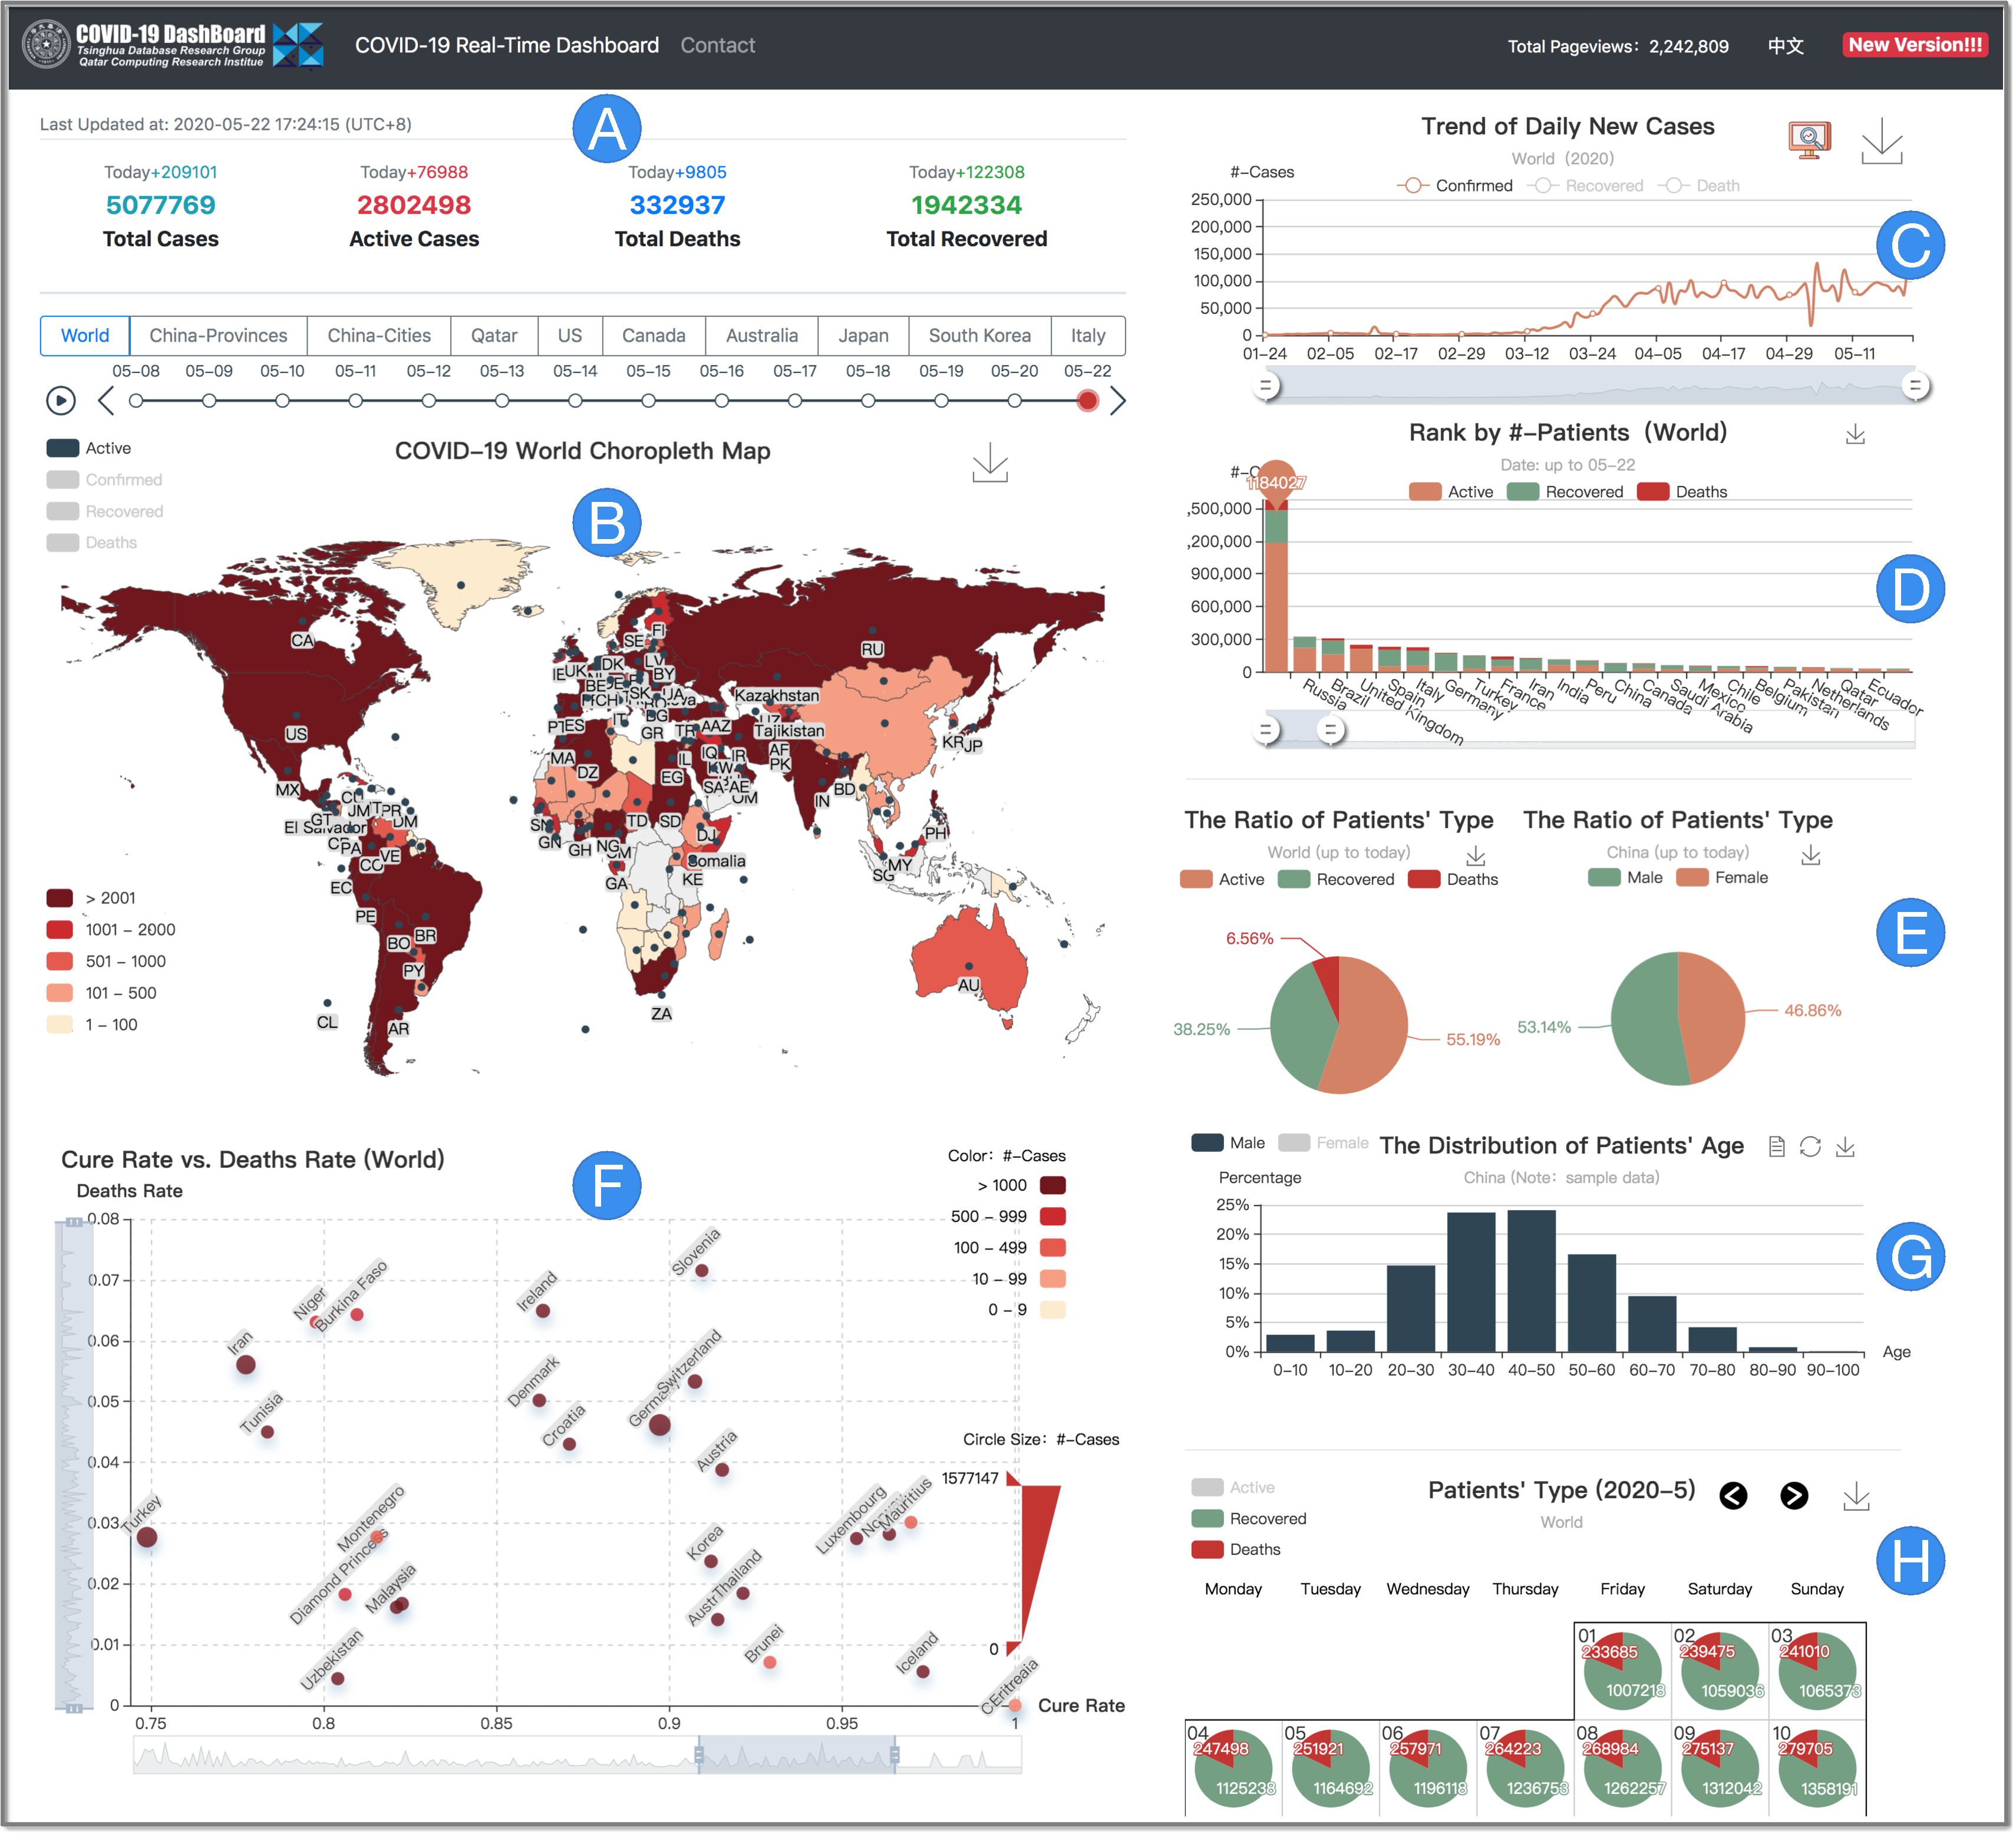
\includegraphics[width=0.9\textwidth]{figs/frontend.pdf}
% 	\caption{Demonstration of \sys-COVID-19 (\lgl{https://ncov.deepeye.tech/en})}
% 	\label{fig:frontend}
% 	\vspace{-.5em}
% \end{figure*}
% %%%%%%%%%%%%%%%%%%%%%%%%%%%%%%%%%%%%






%The data preparation layer, an end-to-end data preparation pipeline, is responsible for collecting, integrating, and cleaning data from multiple data sources. 
%There are some common obstacles in the implementation of this layer. 
%First, we needs to 
%In our application, we collect the reported infected cases from the Chinese Center for Disease Control and Prevention (CDC) and other countries' CDC, and crawler infected cases' age and gender from authoritative news websites, and other data sources like Chinese population statistics.  Moreover, we also gather trajectory data of (potentially) infected persons from China Mobile Limited\footnote{We have collaborated with the company and got mobile phone location data with privacy protection.}. The schema is {\sf S1:}({\sf PhoneID}, {\sf Tag}, {\sf Province}, {\sf City}, {\sf District}, {\sf Address}, { \sf Longitude}, {\sf Latitude}, {\sf Time}).

%Next, we need to integrate different types of data into the relational table.
%For example, we need to extract report date, location, patients' type, \#-cases from each country's CDC's reports, and  perform schema alignment into {\sf S2:}({\sf Date}, {\sf Country}, {\sf State/Province}, {\sf City}, {\sf Total Confirmed}, {\sf Current Confirmed}, {\sf Total Deaths}, {\sf Total Recovered}, {\sf Death Rate}, {\sf Recovered Rate}, {\sf Gender}).

% \stitle{Data Cleaning.} After integrating data from multiple sources, there have typical data errors such as duplicates, missing values, synonyms, and so on. Because data cleaning is known to be tedious and error-prone, we employ our recently proposed technique {\sc VisClean}~\cite{visclean-icde} for visualization-driven data cleaning, which is way cheaper than cleaning the entire dataset. This is doable only after the charts to display have been selected, as discussed below.

%In the above steps, it may introduce some data errors such as duplicates, missing values, and synonyms. 
%Such errors may derive bad visualizations and may misguide users by showing false discoveries. 
%It's necessary to clean the data errors before conduct analysis. However, it is impossible to completely clean a dataset for visualizations (or any other analytical task), simply because data cleaning is prohibitively expensive in terms of the human cost.
%Therefore, we propose to clean those data errors that are relevant to the analysis~\cite{visclean-icde}.

%The system can automatically rerun the pipeline to update data to guarantee its timeliness. 
%Once the pipeline is built, and the data is ready, the next step is to analyze and visualize the data.

% \subsection{Visualization Selection Layer}
% \label{subsec:vs}

% % \add{Paragraph 1: Two types of visualizations are needed. General statistics/trends that can be fixes, and data-driven interesting charts that may be different everyday. So you have Sections 2.2.1 and 2.2.2.}

% Visualization selection generates three categories of charts: {\em linked} common visualizations, {\em ad-hoc} visualizations, and {\em recommended} visualizations.

% \stitle{Linked Common Visualizations.} There are common visualizations for spatial-temporal data exploration, such as a choropleth map (a heat map on a map), line charts to show various trends, bar charts to show the comparison between various groups, scatter charts (or bubble charts) to quantify the relationship between two quantitative variables (\eg death rate vs. cure rate).
% We carefully selected charts (see Figure~\ref{fig:frontend}) that can attract a wide range of interest, and make them ``linked'', \eg when one zoom in from a world level to a country level, all the other charts will be zoomed in, so as to provide a synchronized view from multiple charts.

%%%%%%%%%%%%%%%%%%%%%%%%%%%%%%%%%%%%
\begin{figure}[t!]
	\centering
	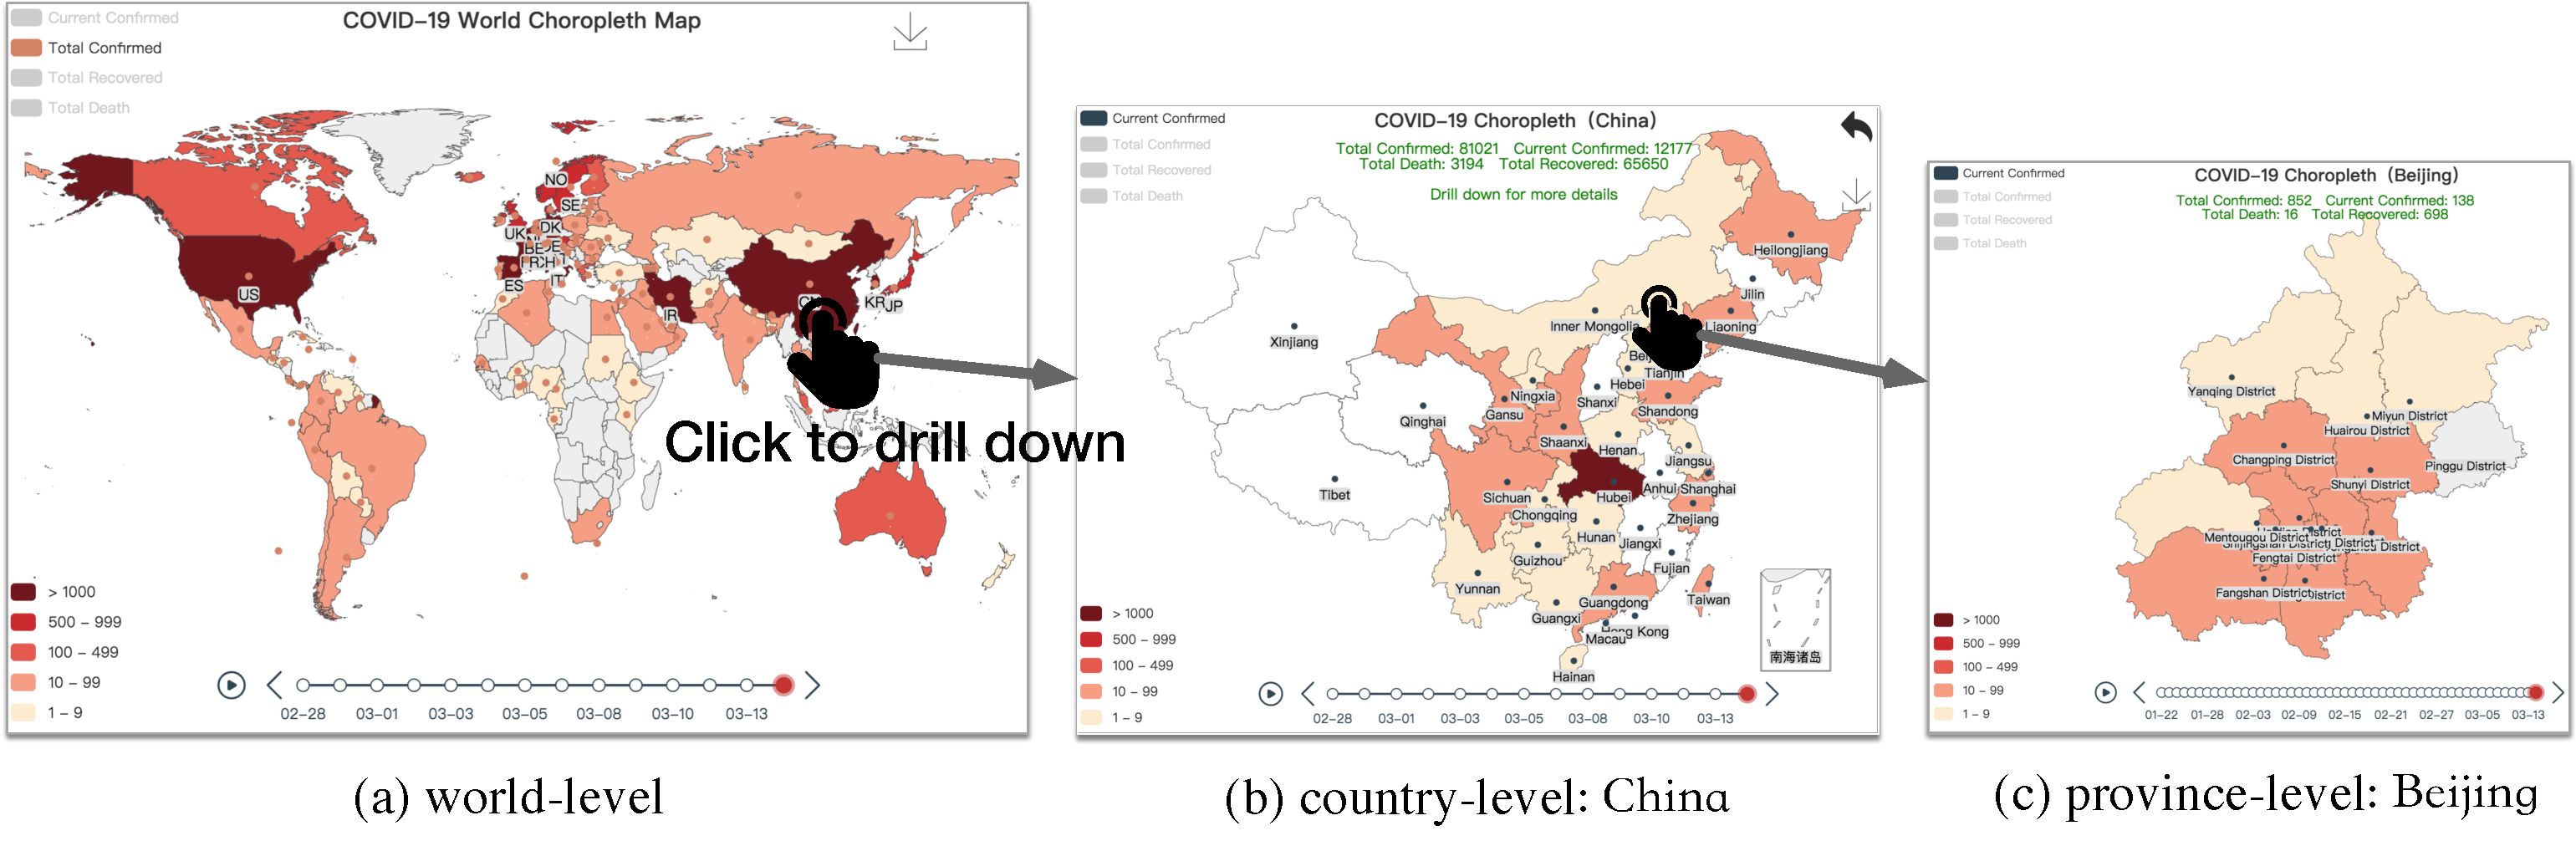
\includegraphics[width=.9\columnwidth]{figs/drill_down_new.pdf}
	\vspace{-1.5em}
	\caption{Drill Down Operation}
	\label{fig:drill_down}
	%	\vspace{-1.5em}
\end{figure}
%%%%%%%%%%%%%%%%%%%%%%%%%%%%%%%%%%%%



\subsection{User Interaction Layer}
\label{subsec:ie}
This is the interface we present to the public.
When a user visits \sys, he/she can further explore visualizations by interactive module for finding more interesting insights. \sys supports popular interactions such as drilling down/up, zooming in/out and linked visualizations, powered by the visualization library ECharts~\cite{DBLP:journals/vi/LiMSSZWZC18}.

Take drill down as an example (see Figure~\ref{fig:drill_down}), when a user clicks a country (\eg China) on the world-level map, the map will drill down into the country-level map for more details.
Note that, \sys provides linked visualizations of the analytical results. That is, when a user performs a drill down operation, other visualizations will also drill down into certain level automatically. In addition, the user can zoom in/out the map by rolling up/down the mouse. 



%It consists of two components, \ie data-dependent visualization design and visualization recommendation. The key points in this layer are (1) what types of visualizations should be designed to interpret the underlying data best; and (2) how to generate such visualizations effectively because there 

% \subsubsection{Data-dependent  Visualization Design}
% For temporal data, there are several common types of visualizations are needed.
% The first type of visualization is line chart, it shows the trend of the temporal data. The second one is bar chart, it shows the distribution or compared information of variables of temporal data, \eg the distribution of the patients' ages.
% Scatter chart (or bubble chart) discovers and quantifies the relationships between two quantitative variables, \eg the death rate v.s. cure rate. 


% \add{Paragraph 1: Maybe you should not call it analysis models, which is not very informative. It should be something like data-dependant chart design or selection, from common ones to special ones, such as infection path or location-based search.}

% It includes a set of data analytical models to process the data for visualization. The analytical models take data as input and output analytical for visualization.
% We implement four types of analysis models in the system. 
% Note that data analysts can plug their analytical model with their domain knowledge into the system, \eg mining the relationships between death rate and medical resources.

% \stitle{Aggregation Analysis.}
% We apply the aggregation analysis to aggregate relational data for visualization. For example, we can use compute the total confirmed cases for each country.

% \stitle{Correlation Analysis.}
% It discovers and quantifies the relationships between two quantitative variables. For example, we can analyze the relationships between \#-cases and recovery (death) rate.

% \stitle{Trend Analysis.}
% For one thing, it records the trend of variables. For another, it can try to predict what will happen in the future.
% In our scenario, we can show the trend of daily increased cases for each country and predict the trend for the coming days. In our system, we use a two-layer neural network $f$ to predict the number of daily confirmed cases in China. The incubation period of the corona virus is 14 days, so we choose the data from the previous 14 days $x=\{c_{-1},c_{-2},...,c_{-14}\}$ as the first input feature and the date of the next day $d$ as the second input feature. We predict the total number of confirmed cases $c = f (x, d)$ the next day. Inspired by the traditional infectious disease model SIR~\cite{kermackcontribution}, we use sigmoid as the activation function in our model $f$.  Gradient descent is used to update the parameters of $f$. By continuously taking the predicted value of the next day as an input, we can continuously predict the confirmed cases in the following days.

% \stitle{Ad-hoc Visualizations}. We also design ad-hoc visualizations to answer specific questions. In terms of COVID-19, besides publicly available datasets, we also have private trajectory data of potentially infected persons. Based on which we have designed two map-based visualizations, one to show infection paths of these patients (see Figure~\ref{fig:infection}), and the other to show the level of risk for each area (see Figure~\ref{fig:heatmap}) and thus suggest the authorities to take different anti-epidemic policies for different areas.

%Besides the above four types of common visualizations, we also need to design some visualizations relevant to analysis scenario.
%Since we also collect the trajectory data of (potential) infected persons.
%Therefore, we use the map to visualize the trajectories. It can benefit us to find such potential infected persons visually, and perform a trajectory similarity search to find a set of similar trajectories to the trajectories of (potential) infected persons. Therefore, we can find a set of high-risk groups. Based on the above analysis, we can further compute the level of risk for each area and thus suggest the authorities take different anti-epidemic policies for different areas.


%\subsubsection{Visualization Recommendation}

% \add{Paragraph 1: Emphasize the requirement of daily news, instead of only daily updates. Why it is hard to have daily news -- a large search space. Naturally, we need some recommendation systems to guide us for doing the job, and we use DeepEye.}

% \stitle{Recommended Visualizations}.
% The above common visualizations are fixed, with data being periodically updated. However, because the data keeps changing, and some interesting stories cannot be captured by predefined common visualizations. Hence, it requires some mechanism to discover these new interesting visualizations, either manually or automatically.
% We leverage our previous work, a visualization recommendation system called {\sc DeepEye}~\cite{deepeyeicde}, to recommend interesting visualizations, such as finding cities in China that share similar trends as Wuhan in terms of death rate. 
% The basic idea of {\sc DeepEye} is to take a table as input, enumerates all possible visualizations of the dataset, select those good visualizations by a supervised classification model, and ranks top-$k$ good visualizations by a learning-to-rank model.

%After we know use what types of visualizations to interpret the data, the next problem is how to process the data for visualization. Not surprisingly, creating good visualizations is not easy in practice, even for the expert. The reason is that it requests the analyst to understand the data both from statistic and semantic perspectives, the right combination of attributes and the right selection of subset. Moreover, the temporal data is usually updated in a certain time interval, and the data feature may also be changed. Thus, the goodness of data-driven visualizations are highly dependent on underlying data.  Therefore, how to select a set of good visualizations after data updating is also a challenge.

%To alleviate the above problem, we propose to use a hybrid method to generate and select good visualizations for the data.  First, we select a set of good visualizations leveraging our previous work, a visualizations recommendation system~\cite{deepeyeicde}. The basic idea of the system is that it takes a relational dataset as input, enumerates all possible visualizations the dataset, select those good visualizations by a classification model, and ranks top-$k$ good visualizations by a learning-to-rank model. Second, we also can manually design good visualizations by incorporating domain knowledge and analysis targets for the dataset. For example, we design a Spatio-temporal choropleth map (\ie choropleth map in Figure~\ref{fig:frontend}) to track the outbreak of COVID-19 around the world visually.  Thus, we select a group of novel visualizations based on the above method and organize those visualizations as a dashboard (See Figure~\ref{fig:frontend}).

% \subsection{Interaction Layer}
% \label{subsec:ie}

% \add{Paragraph 1: You can give some details about the tools you use to implement such a system.}

%Second, what kinds of interactions should we support to enable the visual exploration process more user-friendly.

%\subsection{Interactive Visualization}
%The users also can interact with visualizations to explore the data. 
%
%zoom in, zoom out
%
%drill down, drill up
%
%time line tracking
%
%linking across multiple visualizations

% \stitle{Interaction Types.}

% %%%%%%%%%%%%%%%%%%%%%%%%%%%%%%%%%%%%
% \begin{figure}[t!]
% 	\centering
% 	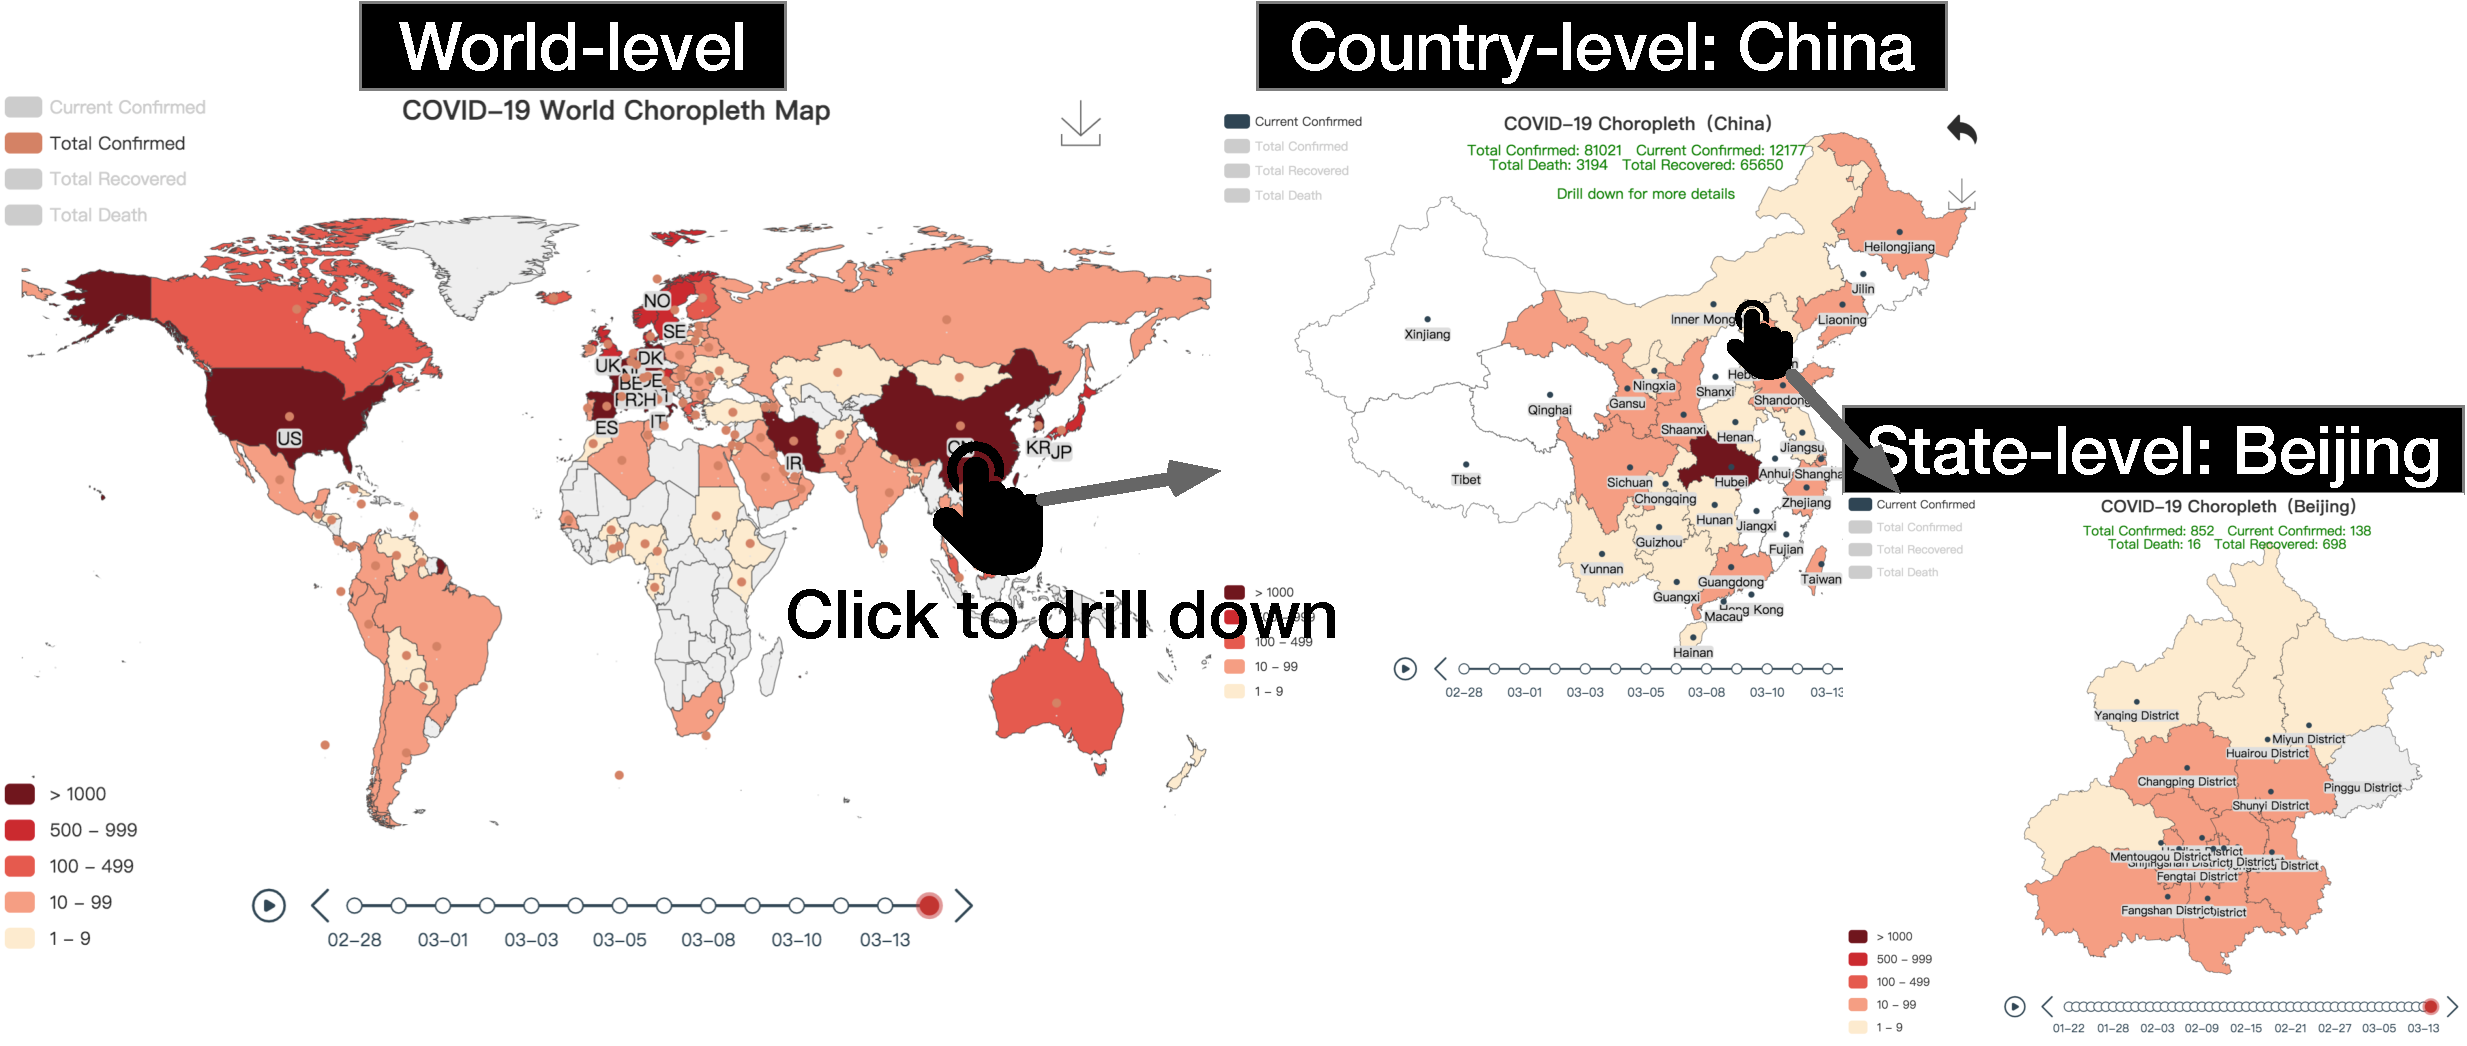
\includegraphics[width=.75\columnwidth]{figs/drill_down.pdf}
% 	\vspace{-1.5em}
% 	\caption{Drill Down Operation}
% 	\label{fig:drill_down}
% %	\vspace{-1.5em}
% \end{figure}
% %%%%%%%%%%%%%%%%%%%%%%%%%%%%%%%%%%%%
% %%%%%%%%%%%%%%%%%%%%%%%%%%%%%%%%%%%%%
% \begin{figure}[t!]
% 	\centering
% 	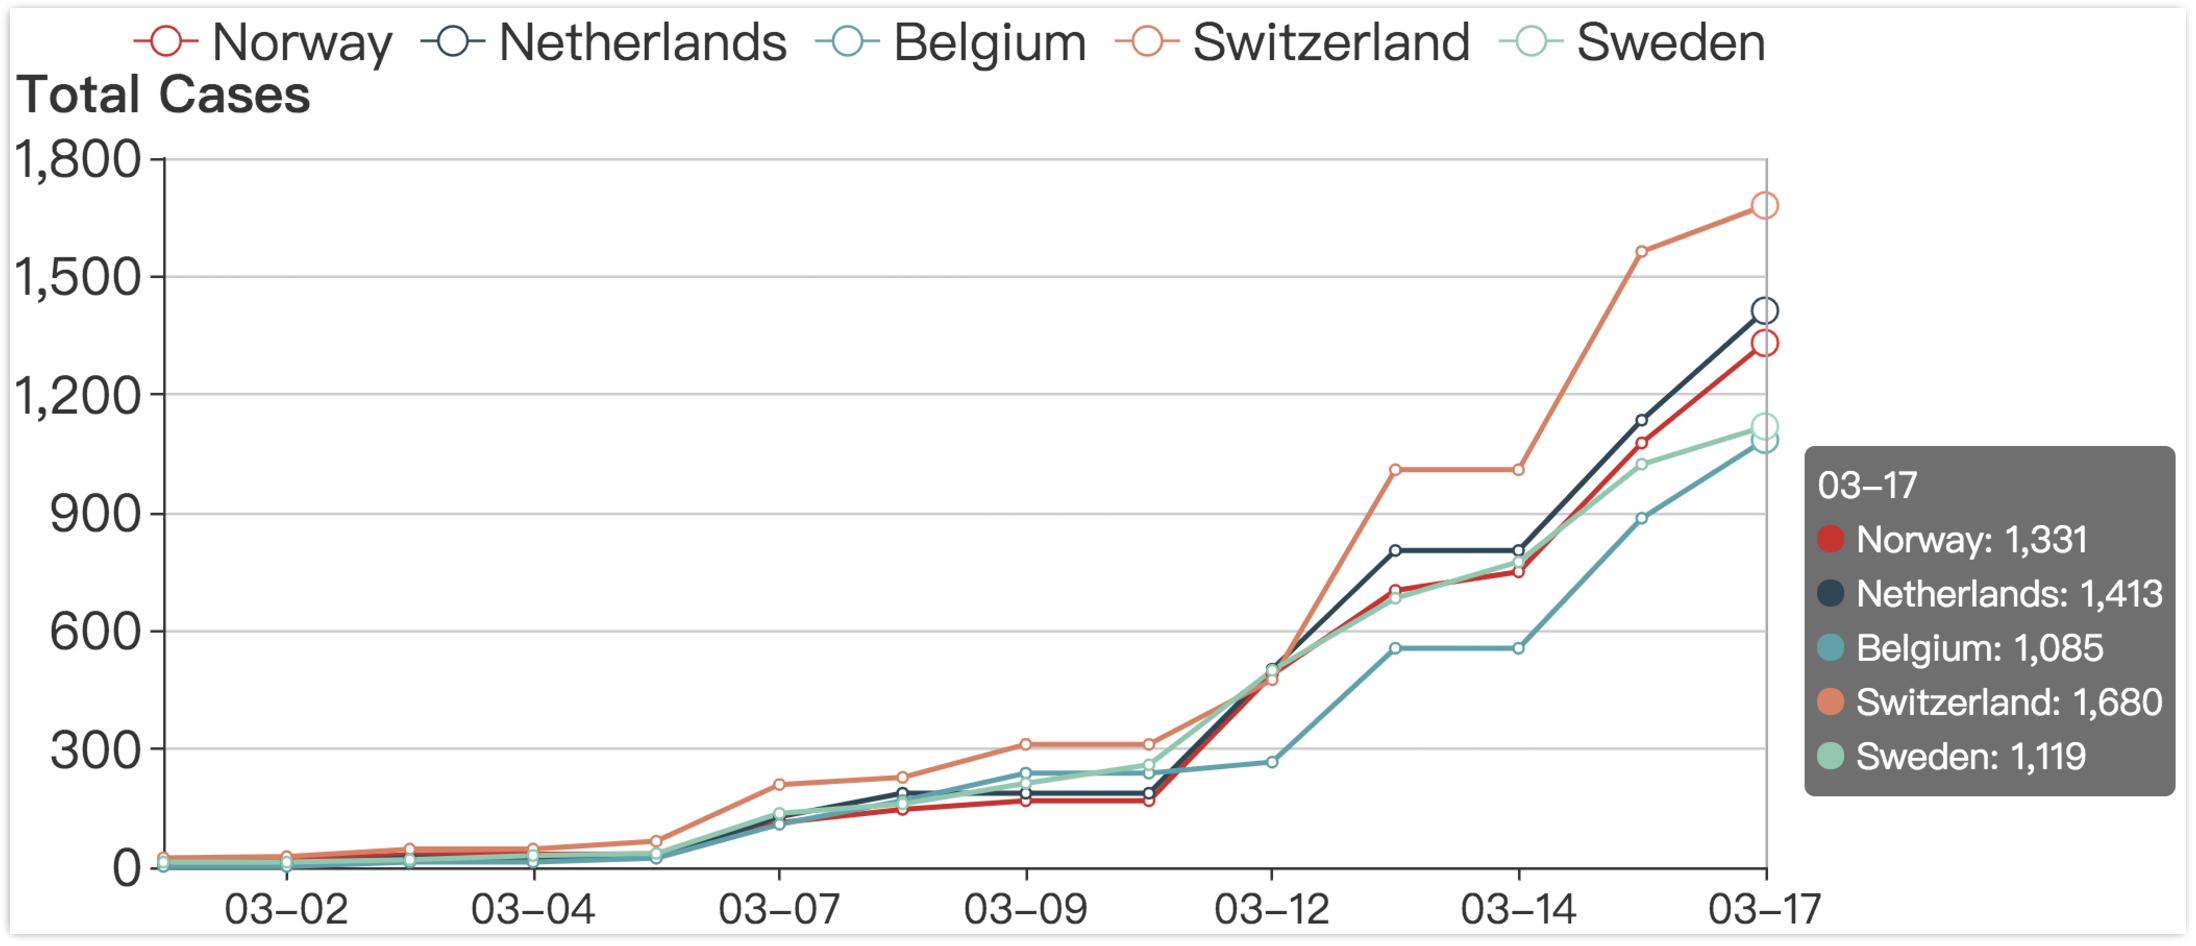
\includegraphics[width=.75\columnwidth]{figs/similarity_trend1.pdf}
% 	\caption{Similar Trend of Confirmed Cases}
% 	\label{fig:similar_trend}
% \end{figure}
% %%%%%%%%%%%%%%%%%%%%%%%%%%%%%%%%%%%%

% \subsection{Interactive Visualization}

% This is the interface we present to the public. 
% When a user visits \sys, he/she can further explore visualizations by interactive module for finding more interesting insights. \sys supports popular interactions such as drilling down/up, zooming in/out and linked visualizations.

% Take drill down as an example (see Figure~\ref{fig:drill_down}), when a user clicks a country (\eg China) on the world-level map, the map will drill down into the country-level map for more details.
% Note that, \sys provides linked visualizations of the analytical results. That is, when a user performs a drill down operations, other visualizations will also drill down into certain level automatically. In addition, the user can zoom in/out the map by rolling up/down the mouse.



% \subsection{How to support reuse and plugin.}
% \label{subsec:disscussion}

